\chapter{Anhang}
\label{chap:anhang}
% Anhänge als \section (Vorlage); je Anhang eine Datei.

\section{Zeichnungen}
\label{sec:anhang_a}
% Inhalt: Rad 2022-03-16, Ritzel 2022-06-23 und 2025-04-02 (30_references_and_examples/93_Zeichnungen).

Die Zeichnungen des Kunststoffrades (Ausgabedatum 28.02.2022) sowie des Stahlritzels (08.06.2022 und 02.04.2025) liegen als Einzelteilzeichnungen der Forschungsstelle vor und sind auf den folgenden drei Seiten wiedergegeben. Die daraus übernommenen Werte nennt \secref{sec:pruefverzahnung}.

% Seiten aus 30_references_and_examples/93_Zeichnungen (Kopien unter bilder/anhang, 2026-10-25); pdfpages lädt die Klasse.
% Maßstab 0,78 und 4 mm nach unten wie die Protokolle in A.7, damit der Zeichnungsrahmen unter der Kopfzeile bleibt (Nutzer, 2026-10-26).
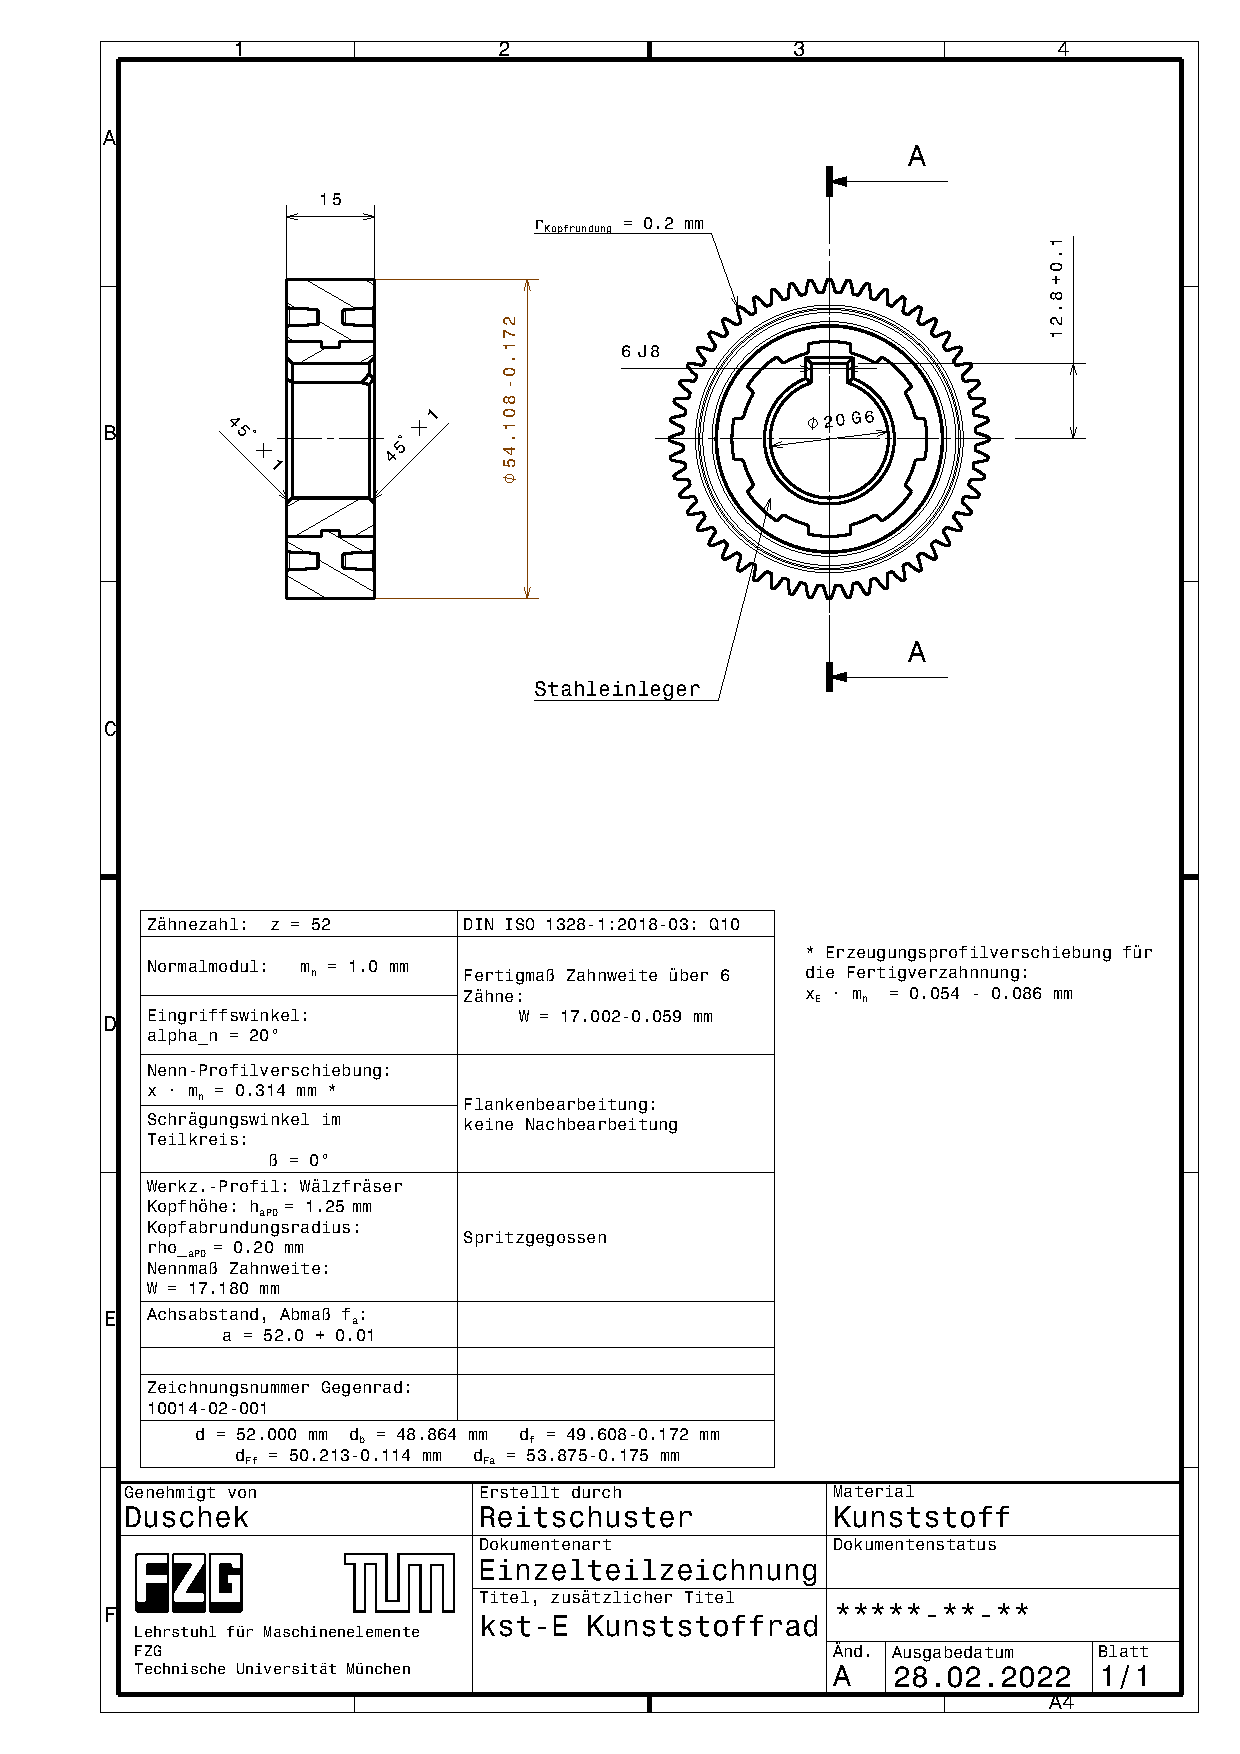
\includepdf[pages=1, scale=0.78, offset=0 -4mm, pagecommand={\thispagestyle{plain}}]{anhang/zeichnung_rad_2022.pdf}
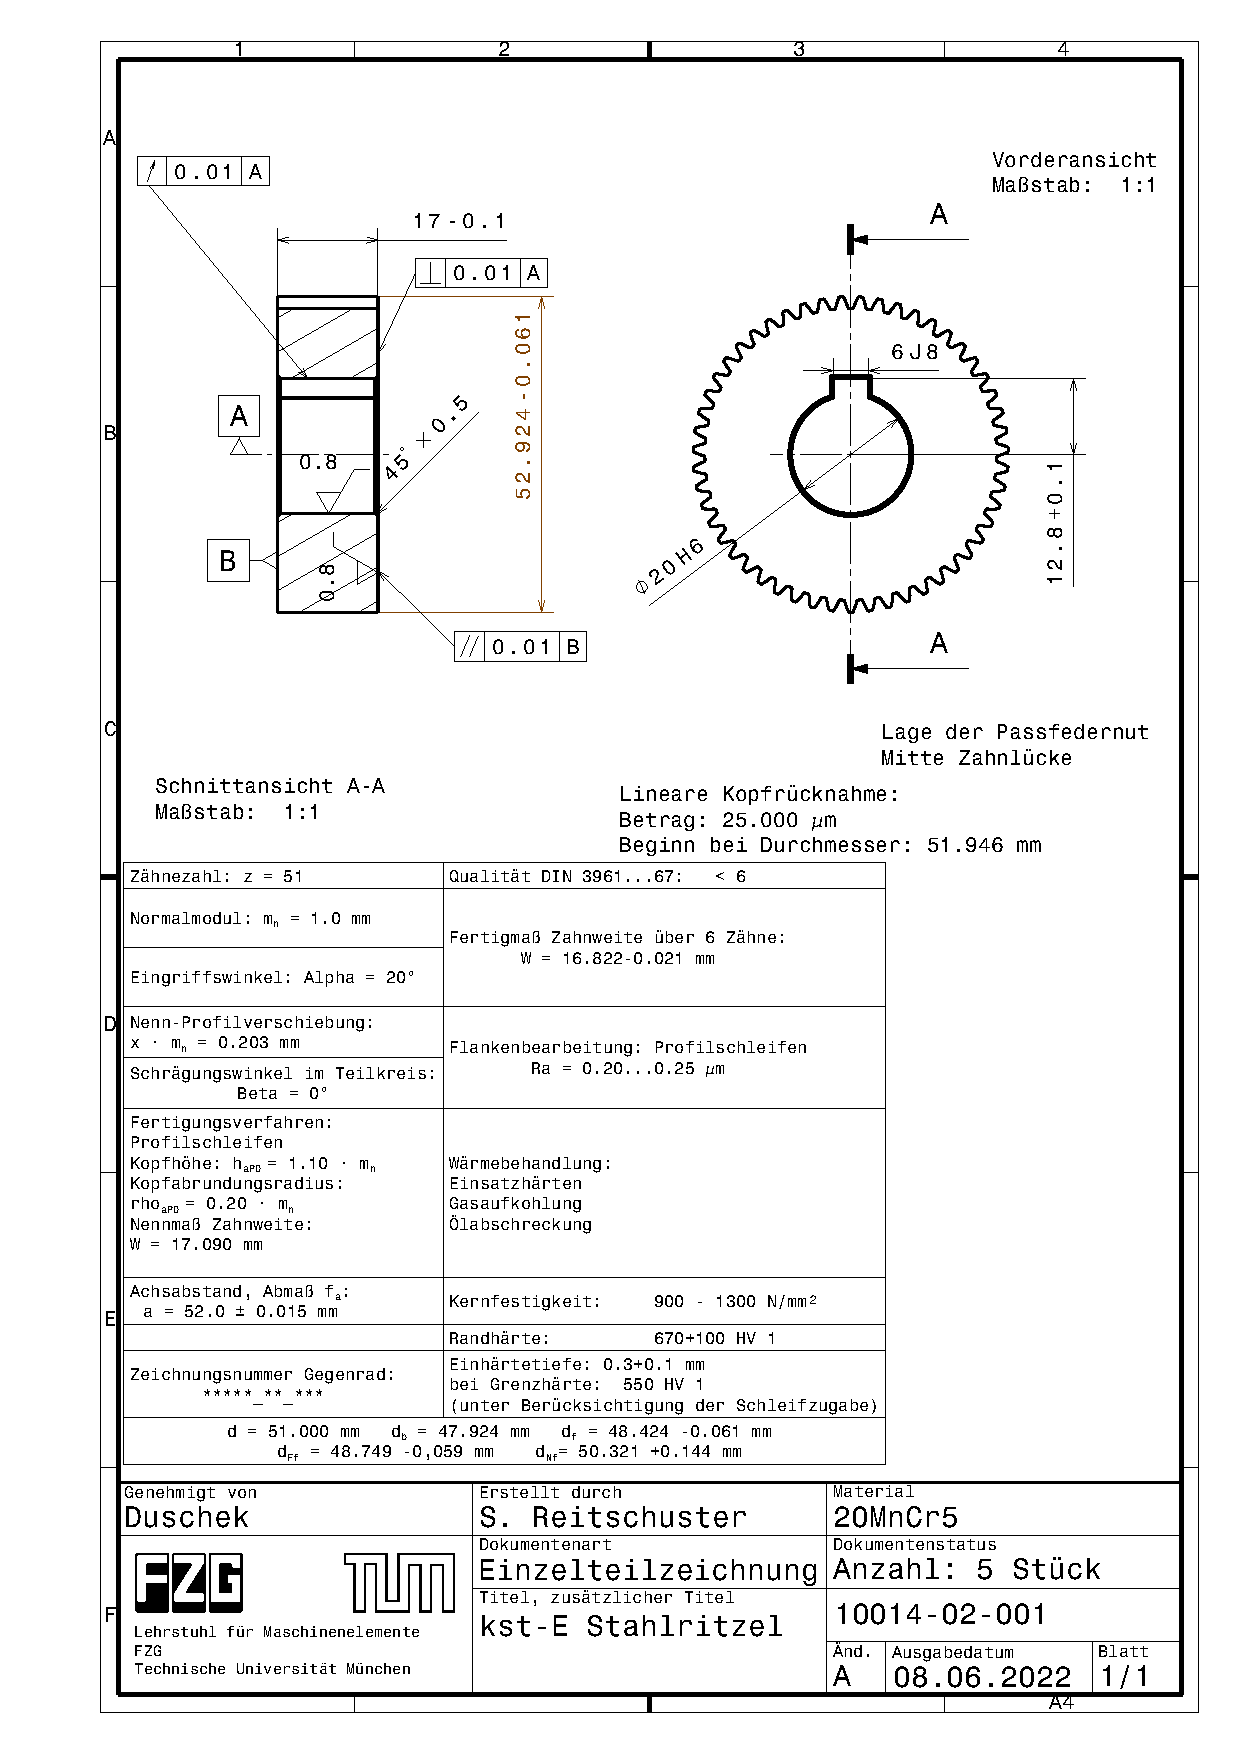
\includepdf[pages=1, scale=0.78, offset=0 -4mm, pagecommand={\thispagestyle{plain}}]{anhang/zeichnung_ritzel_2022.pdf}
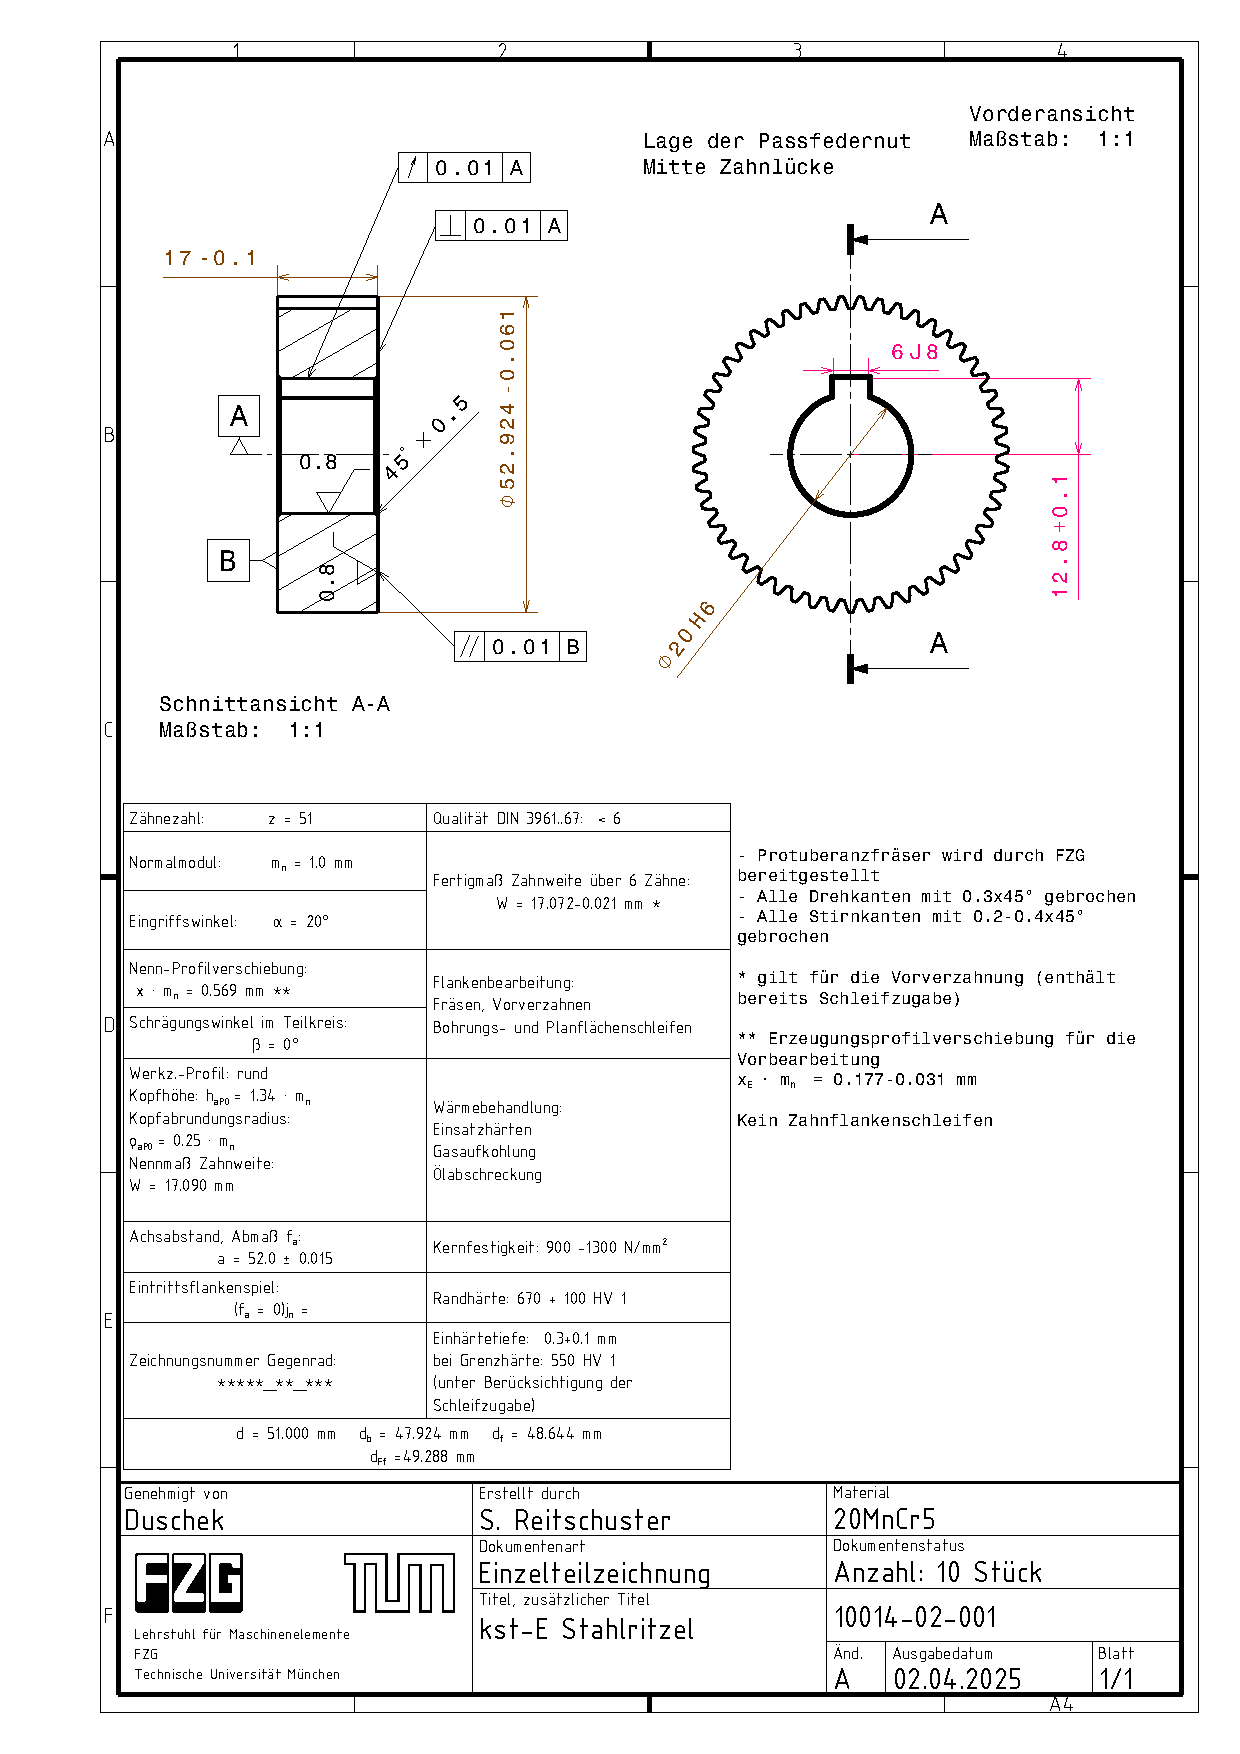
\includepdf[pages=1, scale=0.78, offset=0 -4mm, pagecommand={\thispagestyle{plain}}]{anhang/zeichnung_ritzel_2025.pdf}

\section{Normunterschiede und Geometrietabellen}
\label{sec:anhang_b}
% Inhalt: Tabelle der Unterschiede zwischen den Normen von STplus und den aktuellen Normen (expected_differences.yaml), Geometrietabellen des STplus-Falls kst-E.

\section{Einstellungen des FE-Modells}
\label{sec:anhang_c}
% Inhalt: Netz, Elementtypen je Stufe, Kontakt, Schritte, Iterationsgrenzen, Werkstoffkarten je Rate (simulation_toolchain.md, Manifest der Serie).

\section{Werkstoffkarten und Klassentabellen}
\label{sec:anhang_d}
% Inhalt: Matscape-Karten QS/DY1/DY2 bei 80 °C, Stommel-Klassentabellen, FVA 856 I Tabelle 4.

Die Werkstoffkarten von PA46-GF30 für die quasistatische Belastung und die Dehnraten $3$ und $60$\,1/s bei $23$ und $80$\,\textdegree C liegen als Matscape-Karten mit Rohkurven vor. \secref{sec:materialmodelle} zeigt die Spannungs-Dehnungs-Kurven und die Orientierungszustände, \tabref{tab:fva856_tab4_rt} die elastischen Konstanten der Tabelle 4 aus FVA 856 I. Die Klassentabellen des Nachweises nach Stommel et al. (Tabelle 6.1, Bild 6.18, Bild 6.26, Tabelle 6.3 des Buches) wurden in die Datenbasis übernommen und mit den Zahlenbeispielen des Buches geprüft. Für die drei Karten stellt \tabref{tab:anhang_kennwerte_karten} die Kennwerte bei $23$ und $80$\,\textdegree C zusammen, \tabref{tab:anhang_hill_zustaende} die Hill-Verhältnisse ausgewählter Orientierungszustände bei $80$\,\textdegree C. In \tabref{tab:anhang_klassen_festigkeit} und \tabref{tab:anhang_klassen_abminderung} stehen die Klassentabellen des Buches.

% erzeugt von 20_code/10_gearcore/scripts/thesis_appendix_tables.py, nicht von Hand ändern
\begin{table}[htbp]
    \caption{Kennwerte der Werkstoffkarten von PA46-GF30 (Stanyl TW200F6, konditioniert) für die quasistatische Prüfgeschwindigkeit QS und die Dehnraten DY1 ($3$\,1/s) und DY2 ($60$\,1/s) bei $23$ und $80$\,\textdegree C: die Modelleigenschaften und die Kurven des Zugstabs aus Matscape sowie die isotrope Zeile und der ausgerichtete Zustand der CONVERSE-Karte. Die Streckgrenze ist das Maximum der Kurve in Fließrichtung, der Kennwert $K$ des Nachweises nach Stommel et al.}
    \label{tab:anhang_kennwerte_karten}
    \centering
    \footnotesize
    \setlength{\tabcolsep}{3pt}
    \begin{tabular}{L{2.9cm}lllllll}
        Größe & Einheit & QS $23$\,\textdegree C & QS $80$\,\textdegree C & DY1 $23$\,\textdegree C & DY1 $80$\,\textdegree C & DY2 $23$\,\textdegree C & DY2 $80$\,\textdegree C \\
        \hline
        \arrayrulecolor{black!30}
        \multicolumn{8}{l}{Matscape, Modelleigenschaften} \\
        \hline
        $E_{\mathrm{0}}$ in Fließrichtung & MPa & $5980{,}00$ & $3885{,}64$ & $7589{,}89$ & $4626{,}00$ & $10595{,}59$ & $6074{,}84$ \\
        \hline
        $E_{\mathrm{90}}$ quer zur Fließrichtung & MPa & $3933{,}45$ & $1787{,}00$ & $5390{,}41$ & $2214{,}00$ & $7922{,}89$ & $3290{,}00$ \\
        \hline
        wirksame Orientierung $a_{\mathrm{1}}$ / $a_{\mathrm{2}}$ des Stabs &  & $0{,}698$ / $0{,}238$ & $0{,}698$ / $0{,}238$ & $0{,}698$ / $0{,}238$ & $0{,}698$ / $0{,}238$ & $0{,}698$ / $0{,}238$ & $0{,}698$ / $0{,}238$ \\
        \hline
        \multicolumn{8}{l}{Matscape, Kurven des Zugstabs in Fließrichtung ($0$°) und quer dazu ($90$°)} \\
        \hline
        Streckgrenze $\sigma_{\mathrm{Y}}$, Maximum der Kurve unter $0$° & MPa & $115{,}51$ & $88{,}98$ & $176{,}40$ & $108{,}43$ & $245{,}73$ & $129{,}84$ \\
        \hline
        Dehnung bei $\sigma_{\mathrm{Y}}$, Ende der Kurve & \% & $6{,}36$ & $7{,}00$ & $5{,}24$ & $8{,}28$ & $4{,}60$ & $5{,}02$ \\
        \hline
        Maximum der Kurve unter $90$° & MPa & $70{,}92$ & $52{,}12$ & $104{,}93$ & $62{,}45$ & $135{,}66$ & $75{,}52$ \\
        \hline
        Dehnung beim Maximum unter $90$° & \% & $7{,}96$ & $8{,}21$ & $5{,}88$ & $12{,}76$ & $3{,}46$ & $9{,}88$ \\
        \hline
        \multicolumn{8}{l}{CONVERSE-Karte, isotrope Zeile $a_{11} = a_{22} = 1/3$} \\
        \hline
        $E$ & MPa & $4110{,}21$ & $2282{,}08$ & $5057{,}26$ & $2542{,}51$ & $7916{,}38$ & $3596{,}61$ \\
        \hline
        $\nu$ &  & $0{,}3032$ & $0{,}2997$ & $0{,}3019$ & $0{,}2951$ & $0{,}3061$ & $0{,}2973$ \\
        \hline
        \multicolumn{8}{l}{CONVERSE-Karte, ausgerichteter Zustand $a_{11} = 1$} \\
        \hline
        $E_{\mathrm{1}}$ & MPa & $8962{,}45$ & $5833{,}95$ & $11094{,}46$ & $7159{,}98$ & $14327{,}24$ & $9260{,}83$ \\
        \hline
        $E_{\mathrm{2}}$ & MPa & $3183{,}28$ & $1600{,}12$ & $3874{,}73$ & $1621{,}15$ & $6707{,}62$ & $2459{,}90$ \\
        \hline
        $G_{\mathrm{12}}$ & MPa & $1181{,}97$ & $591{,}25$ & $1433{,}49$ & $595{,}05$ & $2498{,}02$ & $904{,}59$ \\
        \hline
        \arrayrulecolor{black}
    \end{tabular}
\end{table}

% erzeugt von 20_code/10_gearcore/scripts/thesis_appendix_tables.py, nicht von Hand ändern
\begin{table}[htbp]
    \caption{Hill-Verhältnisse $R_{11}$ bis $R_{23}$ der CONVERSE-Karten bei $80$\,\textdegree C für ausgewählte Orientierungszustände $(a_{11}, a_{22})$ des Gitters der Karte, vom isotropen Zustand bis zum ausgerichteten, sowie das Mittel der an den Knoten interpolierten Verhältnisse der Zuordnung auf den Taschenkörper. Die Verhältnisse skalieren die Fließfläche gegen die Bezugskurve des Zugstabs \cite{AbaqusHill25}.}
    \label{tab:anhang_hill_zustaende}
    \centering
    \footnotesize
    \setlength{\tabcolsep}{4pt}
    \begin{tabular}{llllllll}
        $a_{11}$ & $a_{22}$ & $R_{11}$ & $R_{22}$ & $R_{33}$ & $R_{12}$ & $R_{13}$ & $R_{23}$ \\
        \hline
        \arrayrulecolor{black!30}
        \multicolumn{8}{l}{Karte QS (PA46\_GF30\_QS\_cond\_aniso)} \\
        \hline
        $0{,}333$ & $0{,}333$ & $0{,}6835$ & $0{,}6832$ & $0{,}6832$ & $0{,}5057$ & $0{,}5057$ & $0{,}5056$ \\
        \hline
        $0{,}500$ & $0{,}250$ & $0{,}7951$ & $0{,}6358$ & $0{,}6358$ & $0{,}5294$ & $0{,}5294$ & $0{,}4705$ \\
        \hline
        $0{,}500$ & $0{,}000$ & $0{,}8283$ & $0{,}8283$ & $0{,}5884$ & $0{,}6130$ & $0{,}5242$ & $0{,}5242$ \\
        \hline
        $0{,}583$ & $0{,}083$ & $0{,}8693$ & $0{,}6908$ & $0{,}5693$ & $0{,}5772$ & $0{,}5323$ & $0{,}4662$ \\
        \hline
        $0{,}625$ & $0{,}000$ & $0{,}9292$ & $0{,}7327$ & $0{,}5764$ & $0{,}6149$ & $0{,}5571$ & $0{,}4844$ \\
        \hline
        $0{,}750$ & $0{,}000$ & $1{,}0392$ & $0{,}6446$ & $0{,}5703$ & $0{,}6230$ & $0{,}5955$ & $0{,}4495$ \\
        \hline
        $0{,}875$ & $0{,}000$ & $1{,}1715$ & $0{,}5711$ & $0{,}5596$ & $0{,}6448$ & $0{,}6405$ & $0{,}4184$ \\
        \hline
        $1{,}000$ & $0{,}000$ & $1{,}3846$ & $0{,}5489$ & $0{,}5489$ & $0{,}7154$ & $0{,}7154$ & $0{,}4062$ \\
        \hline
        \multicolumn{8}{l}{Karte DY1 (PA46\_GF30\_DY1\_cond\_aniso)} \\
        \hline
        $0{,}333$ & $0{,}333$ & $0{,}6337$ & $0{,}6334$ & $0{,}6334$ & $0{,}4688$ & $0{,}4688$ & $0{,}4687$ \\
        \hline
        $0{,}500$ & $0{,}250$ & $0{,}7642$ & $0{,}5773$ & $0{,}5773$ & $0{,}4963$ & $0{,}4963$ & $0{,}4272$ \\
        \hline
        $0{,}500$ & $0{,}000$ & $0{,}8034$ & $0{,}8034$ & $0{,}5748$ & $0{,}5945$ & $0{,}5099$ & $0{,}5099$ \\
        \hline
        $0{,}583$ & $0{,}083$ & $0{,}8505$ & $0{,}6420$ & $0{,}5170$ & $0{,}5522$ & $0{,}5060$ & $0{,}4288$ \\
        \hline
        $0{,}625$ & $0{,}000$ & $0{,}9203$ & $0{,}6916$ & $0{,}5627$ & $0{,}5964$ & $0{,}5487$ & $0{,}4641$ \\
        \hline
        $0{,}750$ & $0{,}000$ & $1{,}0466$ & $0{,}5877$ & $0{,}5160$ & $0{,}6047$ & $0{,}5782$ & $0{,}4084$ \\
        \hline
        $0{,}875$ & $0{,}000$ & $1{,}1982$ & $0{,}5003$ & $0{,}4838$ & $0{,}6284$ & $0{,}6223$ & $0{,}3641$ \\
        \hline
        $1{,}000$ & $0{,}000$ & $1{,}4455$ & $0{,}4717$ & $0{,}4717$ & $0{,}7094$ & $0{,}7094$ & $0{,}3491$ \\
        \hline
        \multicolumn{8}{l}{Karte DY2 (PA46\_GF30\_DY2\_cond\_aniso)} \\
        \hline
        $0{,}333$ & $0{,}333$ & $0{,}6277$ & $0{,}6274$ & $0{,}6274$ & $0{,}4644$ & $0{,}4644$ & $0{,}4643$ \\
        \hline
        $0{,}500$ & $0{,}250$ & $0{,}7666$ & $0{,}5678$ & $0{,}5678$ & $0{,}4937$ & $0{,}4937$ & $0{,}4202$ \\
        \hline
        $0{,}500$ & $0{,}000$ & $0{,}8081$ & $0{,}8081$ & $0{,}5745$ & $0{,}5980$ & $0{,}5115$ & $0{,}5115$ \\
        \hline
        $0{,}583$ & $0{,}083$ & $0{,}8582$ & $0{,}6367$ & $0{,}5135$ & $0{,}5531$ & $0{,}5076$ & $0{,}4256$ \\
        \hline
        $0{,}625$ & $0{,}000$ & $0{,}9319$ & $0{,}6893$ & $0{,}5620$ & $0{,}5999$ & $0{,}5528$ & $0{,}4630$ \\
        \hline
        $0{,}750$ & $0{,}000$ & $1{,}0655$ & $0{,}5788$ & $0{,}5142$ & $0{,}6084$ & $0{,}5845$ & $0{,}4044$ \\
        \hline
        $0{,}875$ & $0{,}000$ & $1{,}2247$ & $0{,}4859$ & $0{,}4706$ & $0{,}6329$ & $0{,}6272$ & $0{,}3539$ \\
        \hline
        $1{,}000$ & $0{,}000$ & $1{,}4786$ & $0{,}4570$ & $0{,}4570$ & $0{,}7162$ & $0{,}7162$ & $0{,}3381$ \\
        \hline
        \multicolumn{8}{l}{Mittel über die 83\,650 Knoten des Taschenkörpers, Zuordnung der Karte QS (W3)} \\
        \hline
        $0{,}593$ & $0{,}083$ & $0{,}8779$ & $0{,}6856$ & $0{,}5688$ & $0{,}5785$ & $0{,}5353$ & $0{,}4641$ \\
        \hline
        \arrayrulecolor{black}
    \end{tabular}
\end{table}

% erzeugt von 20_code/10_gearcore/scripts/thesis_appendix_tables.py, nicht von Hand ändern
\begin{table}[htbp]
    \caption{Werkstoffklassen des vereinfachten Festigkeitsnachweises nach Stommel et al.: Schubfestigkeitsfaktor $f_{\tau}$ und Steuergröße $q$ \cite[Tabelle 6.1, S.~323]{Sto18}, Abminderungsfaktor $A_{\mathrm{W}}$ der Wechselfestigkeit bei $N = 10^{7}$ \cite[Bild 6.26, S.~362]{Sto18} und Neigungsexponent $k$ der synthetischen Wöhlerlinie \cite[Tabelle 6.3, S.~371]{Sto18}. Die Klasse amorph (verstärkt) trägt für $f_{\tau}$ und $q$ die Werte der spröden Spalte, weil das Buch keine eigene Spalte dafür führt.}
    \label{tab:anhang_klassen_festigkeit}
    \centering
    \footnotesize
    \setlength{\tabcolsep}{4pt}
    \begin{tabular}{L{3.6cm}L{1.9cm}llL{2.4cm}L{2.6cm}}
        Klasse & Verhalten & $f_{\tau}$ & $q$ & $A_{\mathrm{W}}$ & $k$ \\
        \hline
        \arrayrulecolor{black!30}
        teilkristallin (unverstärkt) & duktil & $0{,}58$ & $0{,}00$ & $0{,}20$ bis $0{,}30$ & $11{,}63$ bis $13{,}39$ \\
        \hline
        amorph (unverstärkt) & spröde & $0{,}74$ & $0{,}52$ & $0{,}17$ bis $0{,}20$ & $11{,}63$ bis $12{,}02$ \\
        \hline
        teilkristallin (verstärkt) & semi-duktil & $0{,}65$ & $0{,}26$ & $0{,}25$ & $15{,}65$ bis $20{,}44$ \\
        \hline
        amorph (verstärkt) & spröde & $0{,}74$ & $0{,}52$ & $0{,}17$ & $11{,}39$ bis $13{,}73$ \\
        \hline
        \arrayrulecolor{black}
    \end{tabular}
\end{table}

% erzeugt von 20_code/10_gearcore/scripts/thesis_appendix_tables.py, nicht von Hand ändern
\begin{table}[htbp]
    \caption{Abminderungsfaktoren $A$ des statischen Nachweises nach Stommel et al. je Werkstoffklasse und Belastungsfall, kleinster und größter Wert \cite[Bild 6.18, S.~346]{Sto18}.}
    \label{tab:anhang_klassen_abminderung}
    \centering
    \footnotesize
    \setlength{\tabcolsep}{4pt}
    \begin{tabular}{L{3.6cm}L{2.4cm}L{2.4cm}L{2.4cm}L{2.4cm}}
        Klasse & einmalig & mehrmalig & langzeitig & wechselnd \\
        \hline
        \arrayrulecolor{black!30}
        teilkristallin (unverstärkt) & $0{,}80$ bis $1{,}00$ & $0{,}60$ bis $0{,}80$ & $0{,}50$ bis $0{,}60$ & $0{,}20$ bis $0{,}30$ \\
        \hline
        amorph (unverstärkt) & $0{,}65$ bis $0{,}80$ & $0{,}50$ bis $0{,}65$ & $0{,}40$ bis $0{,}50$ & $0{,}17$ bis $0{,}20$ \\
        \hline
        teilkristallin (verstärkt) & $0{,}55$ bis $0{,}70$ & $0{,}45$ bis $0{,}55$ & $0{,}35$ bis $0{,}45$ & $0{,}25$ \\
        \hline
        amorph (verstärkt) & $0{,}55$ bis $0{,}70$ & $0{,}45$ bis $0{,}55$ & $0{,}35$ bis $0{,}45$ & $0{,}17$ \\
        \hline
        \arrayrulecolor{black}
    \end{tabular}
\end{table}


\section{Konvergenztabellen}
\label{sec:anhang_e}
% Inhalt: Netzleiter, Extrapolation, Elementtypen (fe_mesh_convergence.md).

\section{Nachtlauf- und Pilottabellen}
\label{sec:anhang_f}
% Inhalt: Tabellen der Piloten und Nachtläufe (fe_simulation_log.md, Auswahl).

Die Piloten und Nachtläufe des FE-Modells sind in einem Tagebuch mit Ordner, Einstellungen, Rechenzeit und Ergebnis je Job festgehalten. \Note{PH: Auswahl der Tabellen (Kopfkontakt 36/54 Reihen mal $0{,}02$/$0{,}05$/$0{,}1$\,mm, Tabelle-4-Varianten, Taschenserie, Fußrundungsvarianten W1 bis W4) aus dem Tagebuch der Simulationen.}

\section{GINA- und Rauheitsprotokolle}
\label{sec:anhang_g}
% Inhalt: Messprotokolle der Prüfräder (Auswahl, inventory.md).

Die Messblätter der Verzahnungsmessung und die gedruckten Rauheitsprotokolle der Prüfräder liegen als PDF vor und sind im Inventar der Messungen nach \secref{sec:dokumentation_pruefraeder} gelistet. Als Beispiel folgt das Messblatt der Verzahnungsmessung des Rades 97364 vom 27.05.2026 mit vier Seiten für die Aufspannfehler-Kompensation, das Profil, die Flankenlinie sowie Teilung und Rundlauf. Dazu kommt das Rauheitsprotokoll der linken Flanke desselben Rades. Die Toleranzen auf dem Messblatt sind die der Qualität 7 nach DIN 3962 (\secref{sec:pruefraeder_vorher}).

Die Konturscans der Räder nach dem Lauf sind in \secref{sec:schadensbilder} ausgewertet. \figref{fig:ueberlagerung_97340_z1} zeigt den Zahn 1 des Rades 97340 vor und nach dem Lauf bei $16$\,Nm in derselben Messebene auf dem Sollzahn. Die Abweichung ist nicht überhöht. Die belastete Flanke rechts ist vom Beginn der Verschleißzone bis zum Kopf zurückgesetzt, die unbelastete Flanke links und beide Fußrundungen decken sich mit dem Scan vor dem Lauf.

\begin{figure}[!htbp]
	\centering
	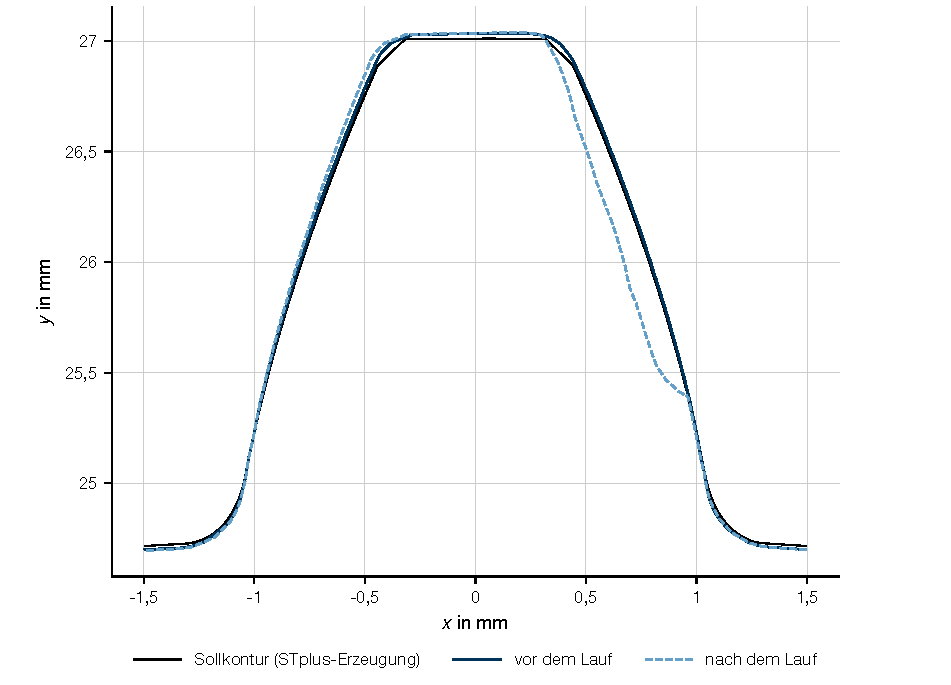
\includegraphics[width=0.8\textwidth]{kap6/ueberlagerung_97340_z1}
	\caption{Zahn 1 des Rades 97340 vor und nach dem Lauf bei $16$\,Nm auf dem Sollzahn der Erzeugung, Messebene $z = 85{,}95$\,mm, Abweichung nicht überhöht.}
	\label{fig:ueberlagerung_97340_z1}
\end{figure}

% Seiten aus 70_input/71_Messungen (Kopien unter bilder/anhang, 2026-10-25): GINA-Messblatt 97364.pdf (4 Seiten), Rauheit 97364-KST_E-li-neu_.pdf.
% Maßstab 0,78 und 4 mm nach unten, damit die Blätter zwischen Kopf- und Fußzeile stehen (Nutzer, 2026-10-26).
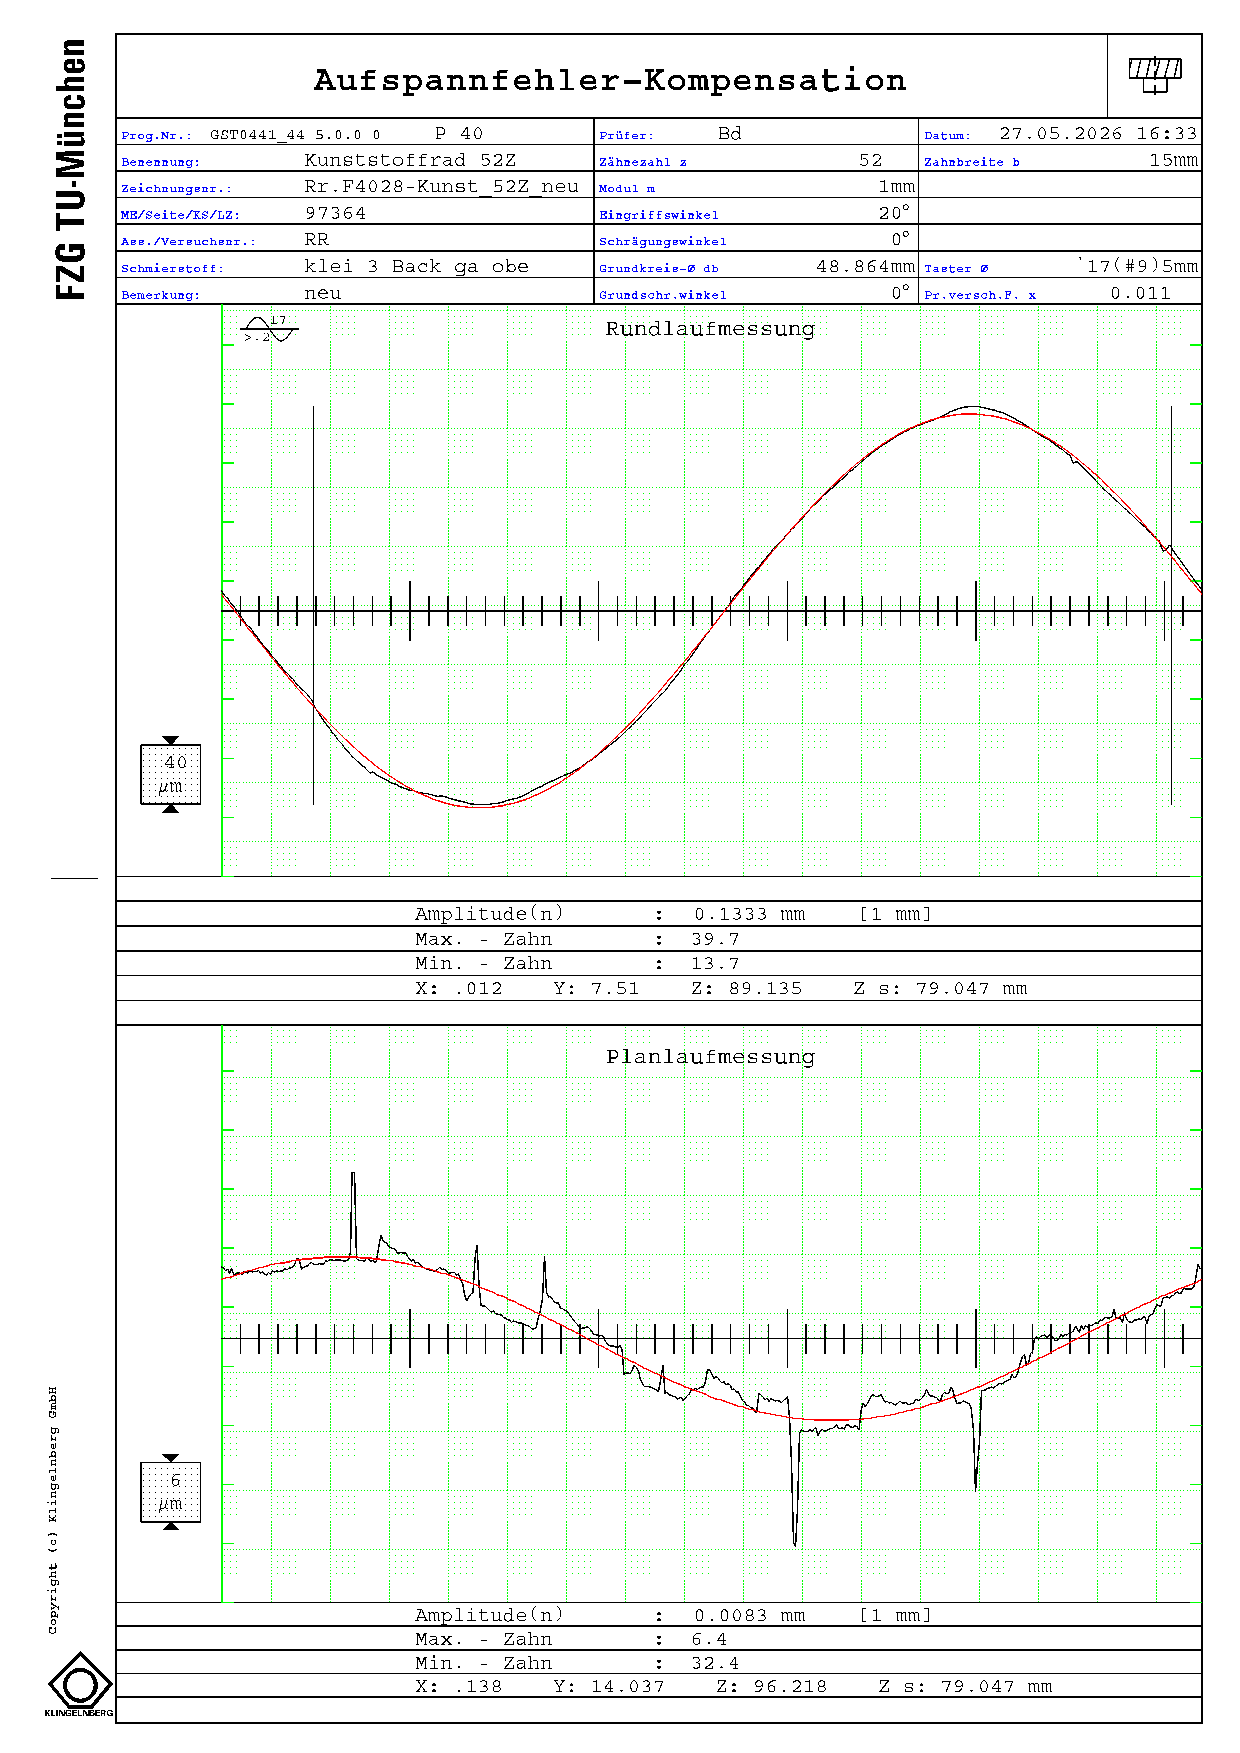
\includepdf[pages=-, scale=0.78, offset=0 -4mm, pagecommand={\thispagestyle{plain}}]{anhang/gina_messblatt_97364.pdf}
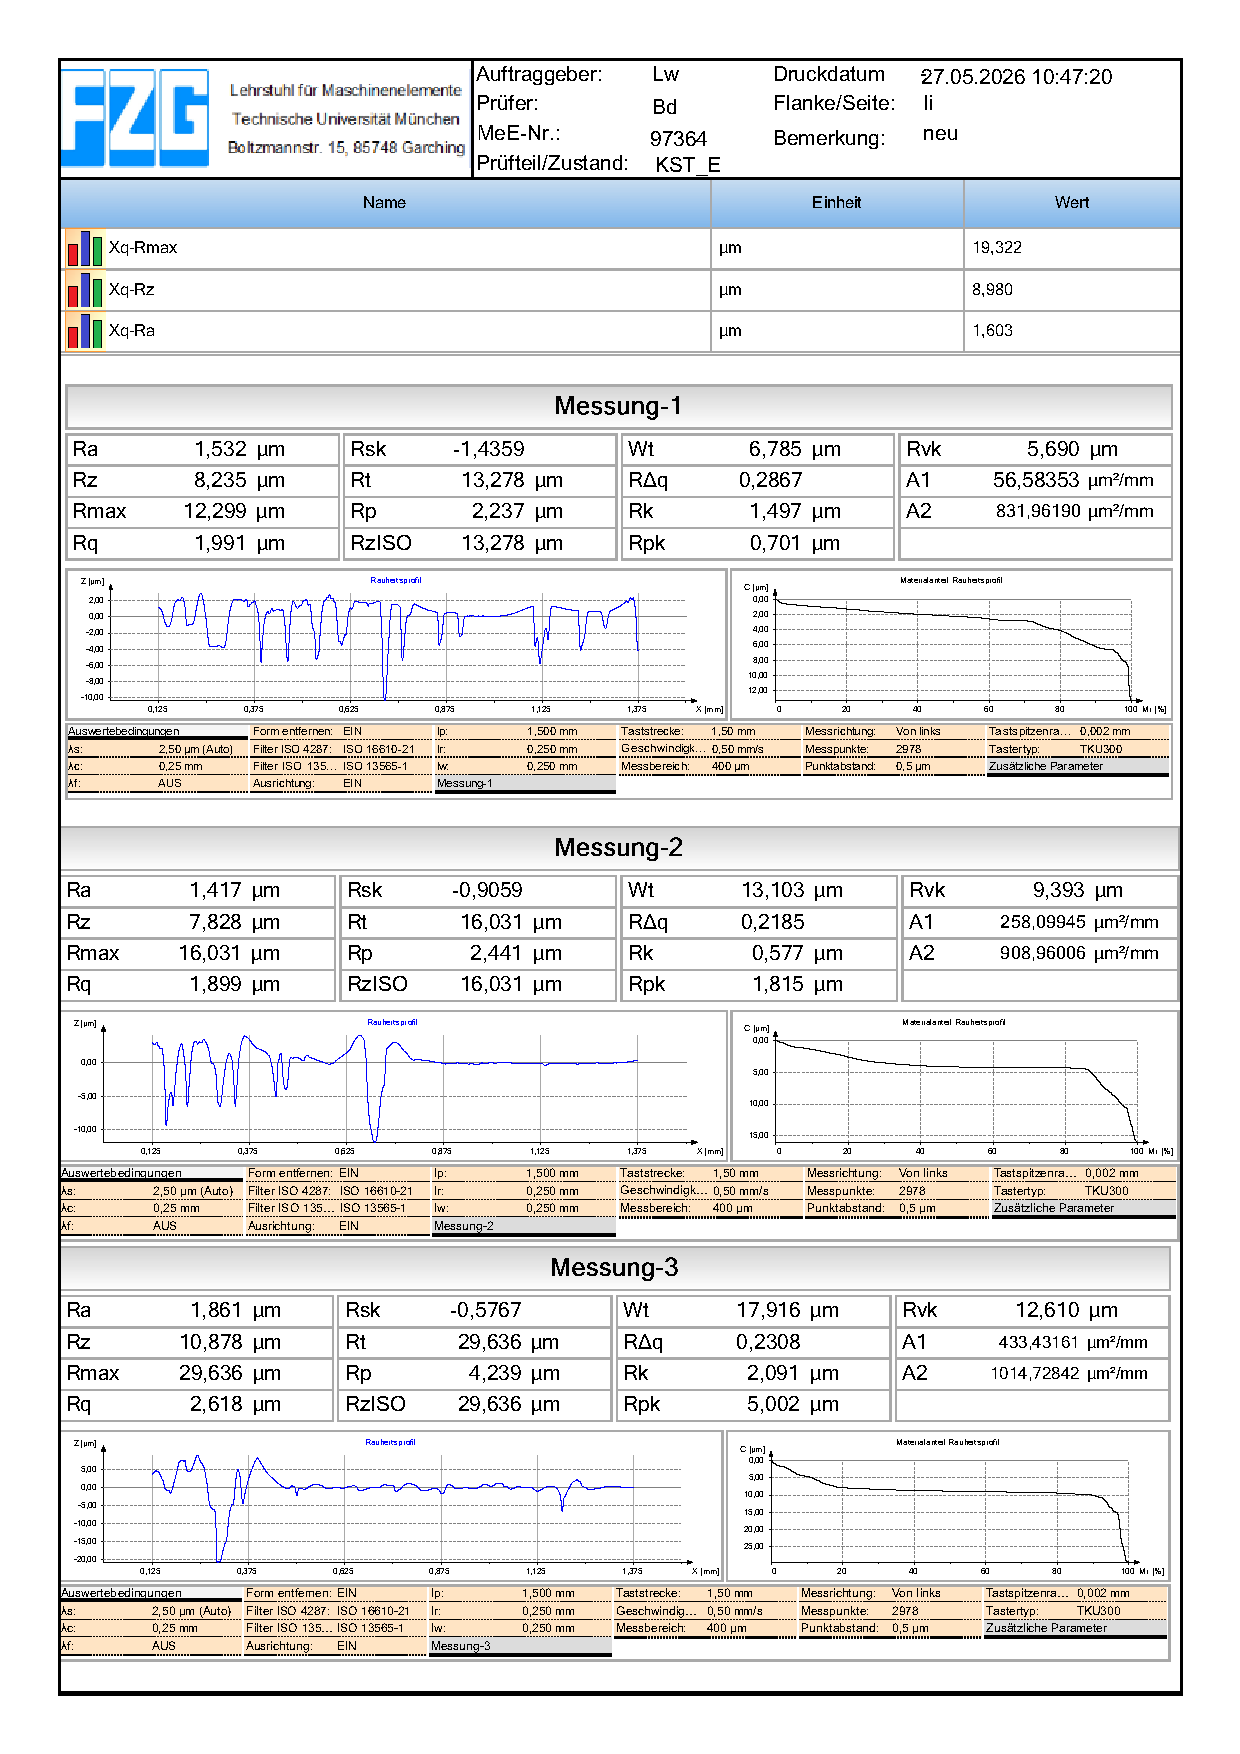
\includepdf[pages=1, scale=0.78, offset=0 -4mm, pagecommand={\thispagestyle{plain}}]{anhang/rauheit_97364_links.pdf}

\section{Prüfstandsprotokoll}
\label{sec:anhang_h}
% Inhalt: Protokoll der Laufversuche (L1).

